%==============================================================================
% Section 7: Reduced orbit atlas and chi-sign separation
%==============================================================================
\section{Reduced orbit atlas and $\chi$-sign separation}
\label{sec:orbit}

\subsection{Derivation of the auxiliary-shell orbit equation}
\label{sec:orbit:derivation}

Taking the lapse variation of the reduced action of
Section~\ref{sec:setup:action} gives the Hamiltonian constraint
\begin{equation}
  \dot q^{2} + F_{\topo}(q,\eta,V;\chi) = 0
  \qquad (N=1\ \text{gauge}),
\end{equation}
with the sign in agreement with
Section~\ref{sec:hamiltonian:constraint}.  The auxiliary fields of each
torsion branch are determined algebraically from
$\delta S/\delta\eta=\delta S/\delta V=0$.  The branch functions used in
this paper are
\begin{equation}
  F_{\EH} = \chi,
  \qquad
  F_{\AX} = \chi - \eta^{2},
  \qquad
  F_{\VT} = \chi + \frac{q^{2}V^{2}}{9},
\end{equation}
\begin{equation}
  F_{\MX}
  = \chi - \eta^{2} + \frac{q^{2}V^{2}}{9}
  + \frac{2}{3} qV\eta\,\kap^{2}\thetaNY.
\end{equation}
The auxiliary equations on $\AX$, $\VT$, and $\MX$ give $\eta=0$, $V=0$,
and $(\eta,V)=(0,0)$, respectively.  On $\MX$ we retain the real-branch
condition of Section~\ref{sec:hamiltonian:constraint}.  Therefore, for all
modes and all topologies,
\begin{equation}
  F_{\topo}\big|_{\text{aux-shell}} = \chi
\end{equation}
holds, and we obtain
\begin{equation}
  \boxed{\,\dot q^{2} + \chi = 0\,}.
\end{equation}
This result is obtained independently of the diagnostic-level bridge result
$\Ctop=-9\chi$ of Section~\ref{sec:pchannel:Pint}, and constitutes the
dynamical-side evidence of $\chi$-universality (see
Section~\ref{sec:bridge:two_appearances}).

\subsection{$\chi$-sign separation}
\label{sec:orbit:sign}

Classifying the auxiliary-shell orbit equation by the sign of $\chi$ gives
Table~\ref{tab:chi_sign_atlas}.

\begin{table}[H]
\centering
\begingroup
\renewcommand{\arraystretch}{2.0}
\begin{tabularx}{\linewidth}{llYY}
\toprule
Sign of $\chi$ & \shortstack{Representative\\topology} & \shortstack{Reduced vacuum\\behaviour} & Notes \\
\midrule
$\chi>0$ & $\Sthree$
         & $\dot q^{2}=-\chi<0$: no real initial data
         & A property of the vacuum orbit, independent of the Hamiltonian admissibility (Table~\ref{tab:four_topology_admissibility}) \\
$\chi=0$ & $\Tthree$
         & $\dot q^{2}=0$: static / degenerate
         & Stability discussion is outside the scope of this paper \\
$\chi<0$ & $\Nilthree$, $\Solthree$
         & $\dot q^{2}=-\chi>0$: monotonic expansion and $q\to 0$ singular-approach collapse
         & Orbit classification within the vacuum reduced atlas of this paper \\
\bottomrule
\end{tabularx}
\endgroup
\caption{$\chi$-sign reduced orbit atlas.}
\label{tab:chi_sign_atlas}
\end{table}

\begin{figure}[H]
  \centering
  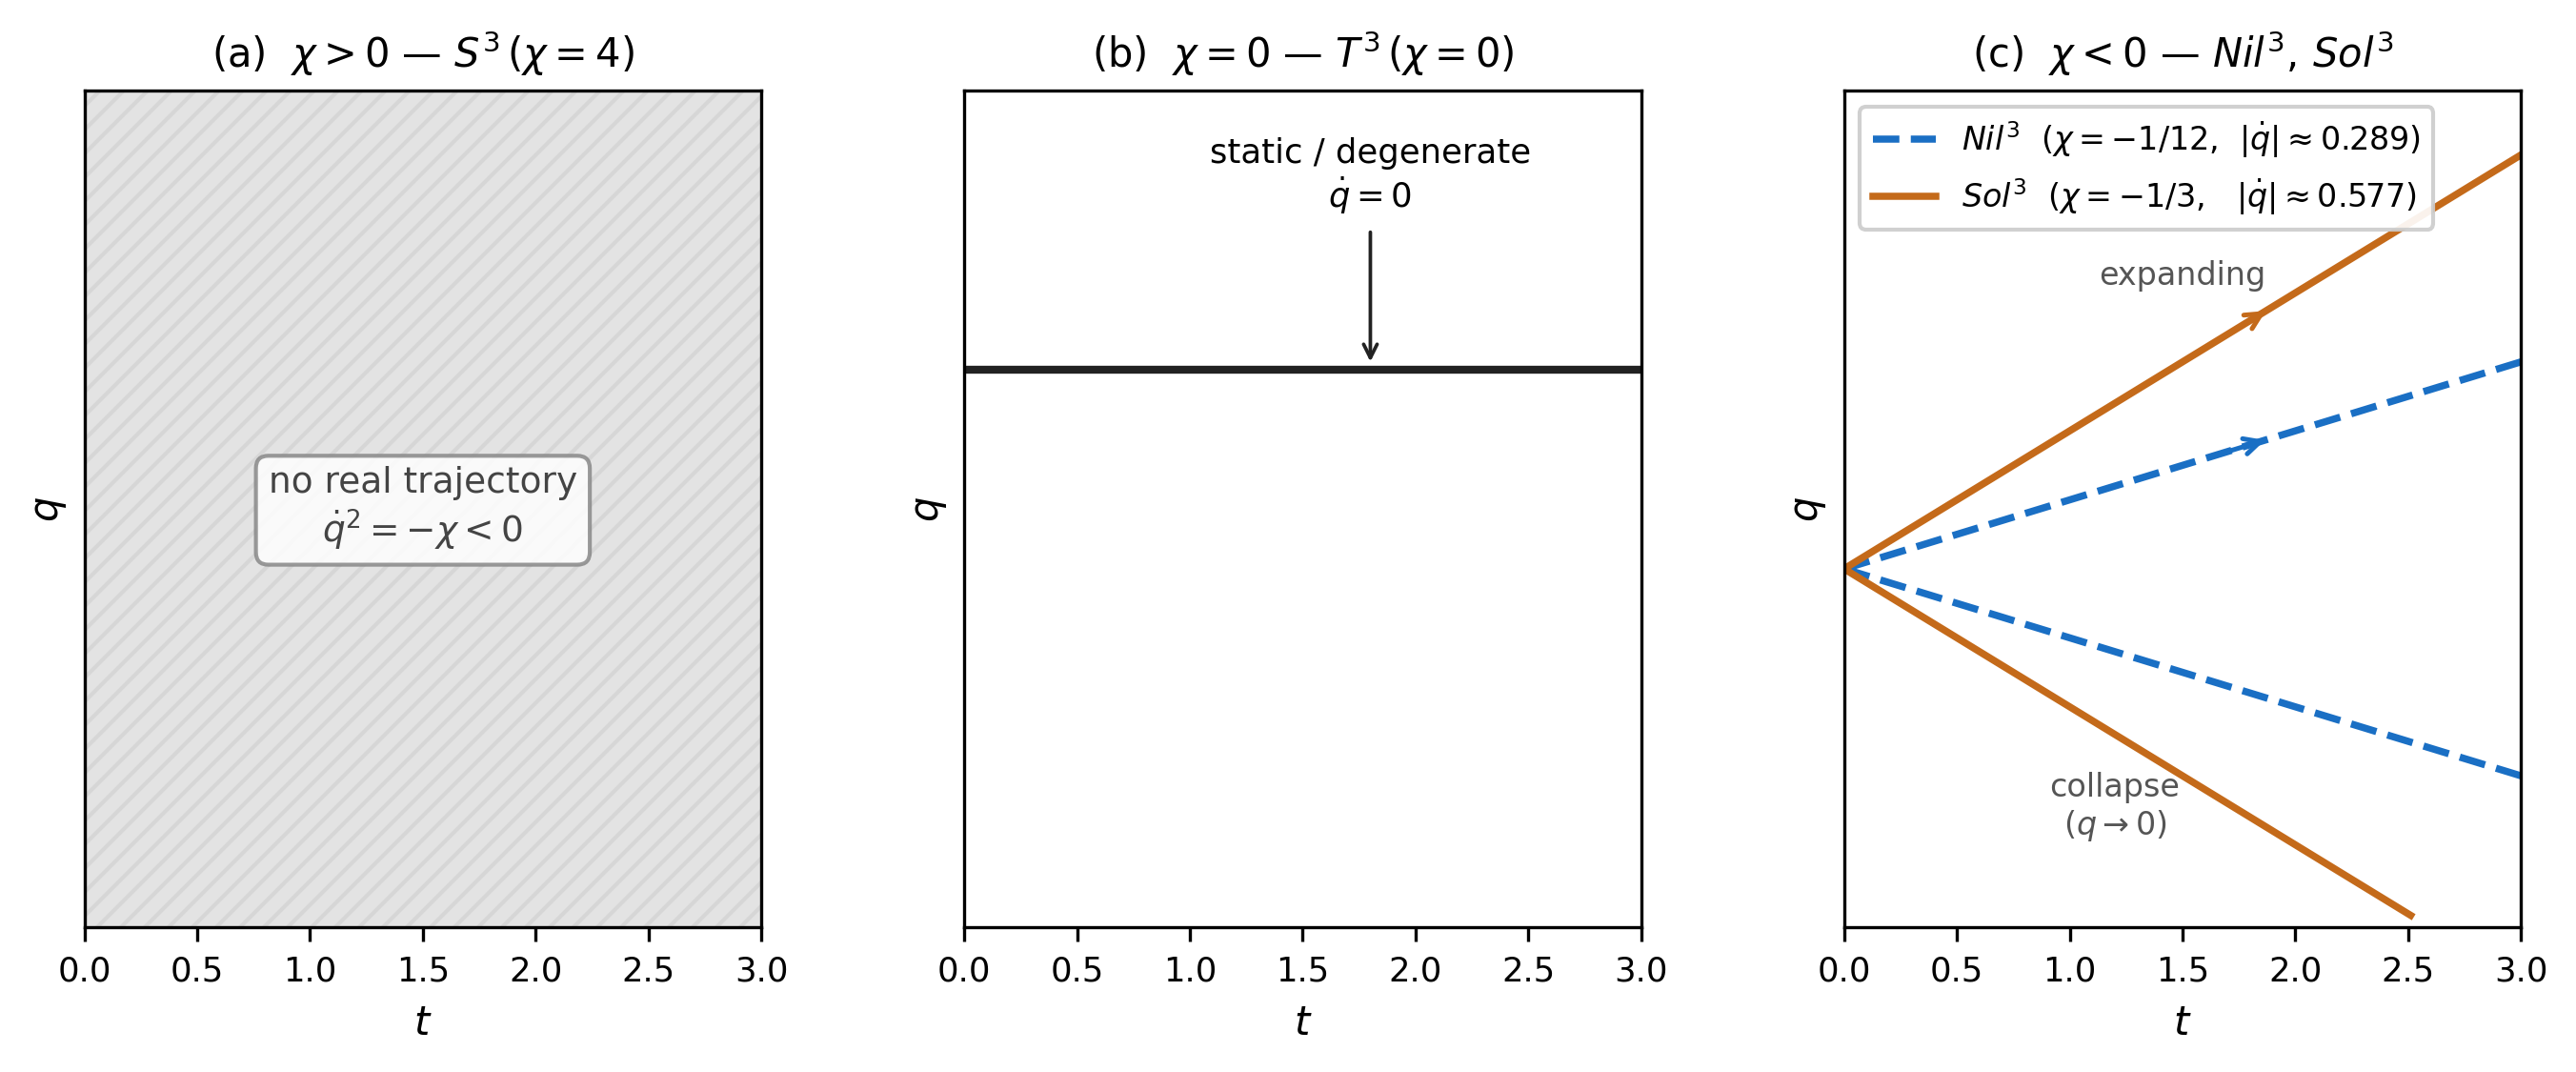
\includegraphics[width=1.0\textwidth]{figures/fig04_chi_sign_orbit_atlas.png}
  \caption{$\chi$-sign reduced orbit atlas, schematic ($q$--$t$ qualitative
    plots).  \textbf{(a) $\chi>0$ ($\Sthree$, $\chi=4$)}: no real initial
    data, since $\dot q^{2}=-\chi<0$ (hatched region).
    \textbf{(b) $\chi=0$ ($\Tthree$, $\chi=0$)}: $\dot q=0$, that is,
    static / degenerate.  \textbf{(c) $\chi<0$ ($\Nilthree$, $\Solthree$)}:
    two sheets $\dot q=\pm\sqrt{-\chi}$ (expanding / collapsing).  The
    slope magnitudes are determined by $|\chi|$:
    $\Nilthree$ gives $|\dot q|=\sqrt{1/12}\approx 0.289$ (dashed) and
    $\Solthree$ gives $|\dot q|=\sqrt{1/3}\approx 0.577$ (solid).
    Bounce-like / recollapse-like classes do not appear in any panel.
    \emph{Caveats}: the figure is a qualitative schematic for the
    constant-velocity solutions of $\dot q^{2}+\chi=0$ and does not include
    an effective potential.  Scope guard: matter coupling, anisotropic, or
    effective-source extensions can change the orbit classes
    (see Section~\ref{sec:orbit:scope} and Appendix~\ref{app:C}).}
  \label{fig:chi_sign_orbit_atlas}
\end{figure}

When $\chi>0$ ($\Sthree$), the absence of real vacuum initial data is a
property of the vacuum reduced atlas, and is independent of the
admissibility classification of
Table~\ref{tab:four_topology_admissibility} (on which $\EH$, $\AX$, $\VT$,
and $\MX$ are all admissible).  The introduction of matter coupling or an
effective source can produce real orbits even on $\Sthree$, but such an
analysis is outside the scope of the present paper.

\subsection{Full-branch sweep summary}
\label{sec:orbit:fullbranch}

The classification of the reduced vacuum orbits across all 16 branches
($\Sthree/\Tthree/\Nilthree/\Solthree$ $\times$ $\EH/\AX/\VT/\MX$) is as
follows.  Each $\chi<0$ branch has two sheets (expanding and collapsing),
so Table~\ref{tab:orbit_class_counts} counts 24 branch/sheet entries
rather than 16 branches.

\begin{table}[H]
\centering
\begin{tabular}{lr}
\toprule
Orbit class & Count \\
\midrule
\code{NO_REAL_AUX_SHELL_ORBIT} & $4$ \\
\code{STATIC_OR_DEGENERATE}    & $4$ \\
\code{MONOTONIC_EXPANSION}     & $8$ \\
\code{SINGULAR_APPROACH}       & $8$ \\
\code{BOUNCE_LIKE}             & $0$ \\
\code{RECOLLAPSE_LIKE}         & $0$ \\
\bottomrule
\end{tabular}
\caption{Full-branch orbit class counts.}
\label{tab:orbit_class_counts}
\end{table}

\code{NO_REAL_AUX_SHELL_ORBIT} reflects the absence of real initial data on
$\Sthree$ ($\chi>0$).  \code{SINGULAR_APPROACH} is the orbit class on the
collapse sheet of $\Nilthree$ and $\Solthree$ ($\chi<0$) for which
$q\to 0$, and is not a statement about finite-time singularities or about
observational cosmology.  Neither class is the same question as the
admissibility classification of
Table~\ref{tab:four_topology_admissibility}.

\subsection{Scope guard}
\label{sec:orbit:scope}

The reduced vacuum atlas considered here contains no \code{BOUNCE_LIKE} or
\code{RECOLLAPSE_LIKE} class.  This is a statement about the vacuum
isotropic reduced setting, and does not extend to matter-coupled,
anisotropic, or effective-source models.  The extensions needed to reach
those settings are discussed in
Section~\ref{sec:discussion:limitations}.
